\documentclass[final]{fhnwreport}       %[mode] = draft or final
                                        %{class} = fhnwreport, article, 
                                        %          report, book, beamer, standalone
%%---Main Packages-----------------------------------------------------------------------
\usepackage[english, ngerman]{babel}	%Mul­tilin­gual sup­port for LaTeX
\usepackage[T1]{fontenc}				%Stan­dard pack­age for se­lect­ing font en­cod­ings
\usepackage[utf8]{inputenc}				%Ac­cept dif­fer­ent in­put en­cod­ings
\usepackage{lmodern}                    %The newer Font-Set
\usepackage{textcomp}					%LaTeX sup­port for the Text Com­pan­ion fonts
\usepackage{graphicx} 					%En­hanced sup­port for graph­ics
\usepackage{float}						%Im­proved in­ter­face for float­ing ob­jects
\usepackage{ifdraft}                    %Let you check if the doc is in draft mode

%%---Useful Packages---------------------------------------------------------------------
\usepackage[pdftex,dvipsnames,table]{xcolor}  %Driver-in­de­pen­dent color ex­ten­sions for LaTeX
\usepackage{csquotes}                   %Simpler quoting with \enquote{}
\usepackage{siunitx} 					%A com­pre­hen­sive (SI) units pack­age
\usepackage{listings}					%Type­set source code list­ings us­ing LaTeX
\usepackage[bottom]{footmisc}			%A range of foot­note op­tions
\usepackage{footnote}					%Im­prove on LaTeX's foot­note han­dling
\usepackage{verbatim}					%Reim­ple­men­ta­tion of and ex­ten­sions to LaTeX ver­ba­tim
\usepackage[textsize=footnotesize]{todonotes} %Mark­ing things to do in a LaTeX doc­u­ment
\usepackage{booktabs}
\usepackage{lscape}
\usepackage{blindtext}
\usepackage{wrapfig}

%%---Tikz Packages-----------------------------------------------------------------------
\usepackage{standalone}
\usepackage{tikz}
\usepackage{circuitikz}
\usetikzlibrary{arrows}
\usetikzlibrary{calc}
\usetikzlibrary{intersections}

%%---Math Packages-----------------------------------------------------------------------
\usepackage{amsmath}					%AMS math­e­mat­i­cal fa­cil­i­ties for LaTeX
%\usepackage{amssymb}					%Type­set­ting symbols (AMS style)
%\usepackage{array}						%Ex­tend­ing the ar­ray and tab­u­lar en­vi­ron­ments
%\usepackage{amsthm}					%Type­set­ting the­o­rems (AMS style)

%%---Table Packages----------------------------------------------------------------------
\usepackage{tabularx}					%Tab­u­lars with ad­justable-width columns
%\usepackage{longtable}
\usepackage{multirow}					%Create tab­u­lar cells span­ning mul­ti­ple rows
\usepackage{multicol}					%In­ter­mix sin­gle and mul­ti­ple columns

%%---PDF / Figure Packages---------------------------------------------------------------
\usepackage{pdfpages}					%In­clude PDF doc­u­ments in LaTeX
\usepackage{pdflscape}					%Make land­scape pages dis­play as land­scape
\usepackage{subfig}					    %Fig­ures di­vided into sub­fig­ures

%%---Other Packages----------------------------------------------------------------------
%\usepackage{xargs}                     %De­fine com­mands with many op­tional ar­gu­ments

%%---Bibliography------------------------------------------------------------------------
%\usepackage[style=ieee,urldate=comp,backend=biber]{biblatex}
\bibliographystyle{IEEEtran}
%\addbibresource{literature/bibliography.bib}

%%---Main Settings-----------------------------------------------------------------------
\graphicspath{{./graphics/}}			%Defines the graphicspath
%\geometry{twoside=false}				    %twoside=false disables the "bookstyle"
\setlength{\marginparwidth}{2cm}
\overfullrule=5em						%Creates a black rule if text goes over the margins => debugging


%%---User Definitions--------------------------------------------------------------------
%%Tabel-Definitions: (requires \usepackage{tabularx})
\newcolumntype{L}[1]{>{\raggedright\arraybackslash}p{#1}}    %column-width and alignment
\newcolumntype{C}[1]{>{\centering\arraybackslash}p{#1}}
\newcolumntype{R}[1]{>{\raggedleft\arraybackslash}p{#1}}

%%---Optional Package Settings-----------------------------------------------------------
%Listings-Settings: (requires \usepackage{listings}) => Example with Matlab Code
\lstset{language=Matlab,%
    basicstyle=\footnotesize\ttfamily,
    breaklines=false,%
    morekeywords={switch, case, otherwise},
    keywordstyle=\color{Blue},%
    tabsize=2,
    %morekeywords=[2]{1}, keywordstyle=[2]{\color{black}},
    identifierstyle=\color{Black},%
    stringstyle=\color{Purple},
    commentstyle=\color{Green},%
    showstringspaces=false,%without this there will be a symbol in the places where there is a space
    numbers=left,%
    numberstyle={\tiny \color{black}},% size of the numbers
    numbersep=9pt, % this defines how far the numbers are from the text
    %emph=[1]{word1, word2,...},emphstyle=[1]\color{red}
}										                %loads all packages, definitions and settings												
\title{\Huge{\textbf{Recherche}}}          %Project Title
\author{\huge{Wetterstation mit Solar Energie}}          %Document Type => Technical Report, ...
\date{Windisch, \today}             %Place and Date


\begin{document}


%%---TITLEPAGE---------------------------------------------------------------------------
\selectlanguage{ngerman}                %ngerman or english
\maketitle
%\vspace*{-1cm}
\vspace*{-0.5cm}						    %compensates the space after the date line.
\vfill
\begin{figure}[H]
\centering
%\includegraphics[width=\linewidth]{Titelbild.jpg}
\end{figure}
\vfill

{
\renewcommand\arraystretch{2}
\begin{center}
\begin{tabular}{>{\bf}p{4cm} l}
Hochschule                 &    Hochschule für Technik - FHNW\\
Studiengang                &    Elektro- und Informationstechnik\\
Autor   		           & 	Andres Minder\\
Betreuer                   &    Prof. Dr. Taoufik Nouri\\
Auftraggeber               &    Prof. Dr. Taoufik Nouri\\
Version                    &    1.0 %Normally not used!
\end{tabular}
\end{center}
}

\clearpage
			
%%---ABSTRACT----------------------------------------------------------------------------
\selectlanguage{english}				%ngerman or english
\thispagestyle{empty}
%\include{sections/abstract}

%%---TABLE OF CONTENTS-------------------------------------------------------------------
\pagenumbering{Roman}		
\selectlanguage{ngerman}				%ngerman or english
\tableofcontents
\clearpage

%%---TEXT--------------------------------------------------------------------------------
\pagenumbering{arabic}
\section{Niederschlag}
Es gibt sehr viele verschiedene Möglichkeiten den Niederschlag zu messen. Aus Rücksicht zum Projekt 5 und deren Umsetzbarkeit wäre es am schlausten die Niederschlagsmessung (elektrisch mit geloggten Daten) als Wunschziel zu definieren. Ein analoges Messverfahren mit einem Füllbecher zur optischen Betrachtung vor Ort wäre also eine Alternative. Anderenfalls könnten, falls alle Sensordaten auf einer Webpage geloggt werden würden, die Niederschlagsdaten von einer offiziellen Wetterseite bezogen werden. Wichtig zur weiteren Betrachtung sind die benötigten/unterstützen Schnittstellen/Protokolle RS-585 und SDI-12. Diese sind für den Datenaustausch der Loggeinheit und des Sensors wichtig.
\subsection{Regenmelder}
\begin{multicols}{2}
{ \centering
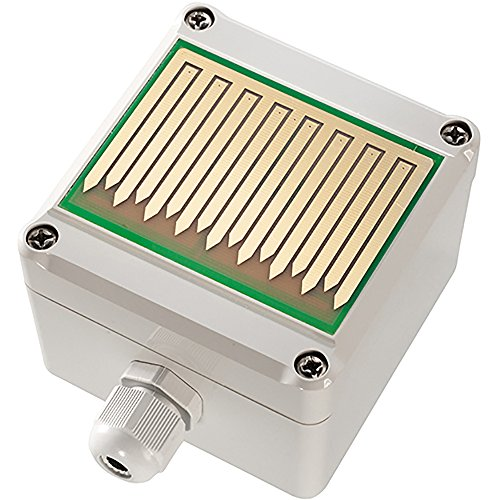
\includegraphics[width=0.4\columnwidth]{graphics/regenmelder.jpg}\\
\captionof{figure}{Regenmelder}
\label{regenmelder}
}
\columnbreak
Es gibt Regenmelder, welche einfach nur den Regen detektieren. Dafür können kapazitive Regensensoren verwendet werden, welche herausfinden ob es regnet oder nicht. Diese müssen seitlich montiert werden, dass das Wasser abläuft und sie müssen zwingend beheizt sein damit der Sensor wieder trocknen kann.
\end{multicols}

\subsection{Niederschlagsmesssensor}
Mit diesem Instrument kann der Niederschlag gemessen werden, welcher in einem bestimmten Zeitintervall gefallen ist (Regen, Schnee wenn dieser zu seinem Wasseräquivalent geschmolzen ist und allenfalls Hagel). Dabei gibt es für dieses Projekt verschiedene Verfahren zur Messung, welche in Frage kommen könnten\footnote{wurden direkt priorisiert}:
\begin{itemize}
\item[1.] Disdrometer
\item[2.] Kippwaage
\item[3.] Wägeprinzip
\end{itemize}
\begin{figure}[hbtp]
\centering
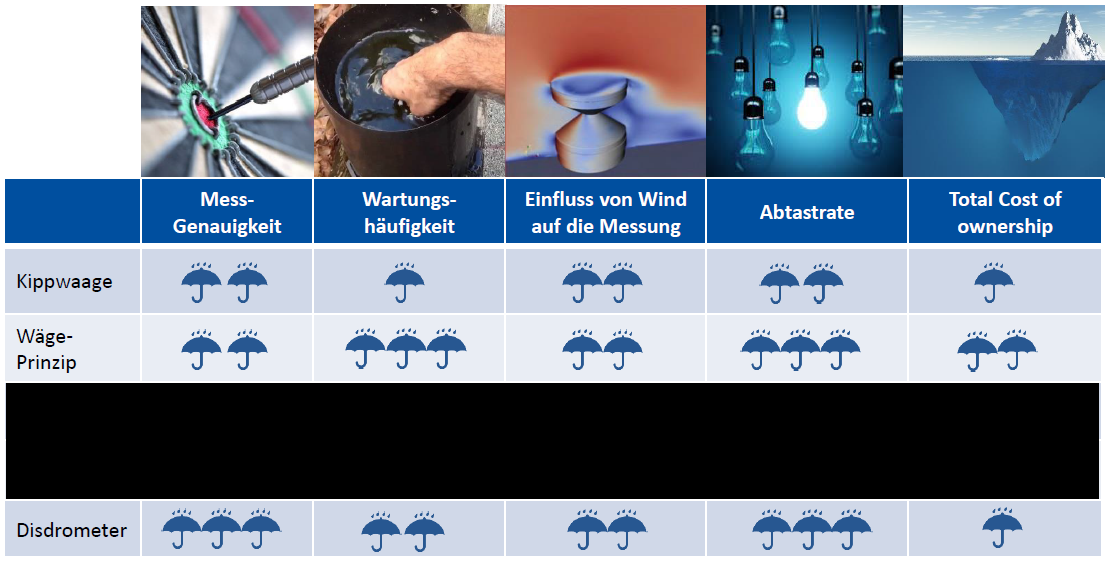
\includegraphics[width=0.85\textwidth]{graphics/vergleich_verfahren.PNG}
\caption{Vergleich der Verfahren}
\label{vergleich_der_verfahren}
\end{figure}

\subsubsection{Disdrometer}
Ein Disdrometer misst im Gegensatz zu den anderen beiden Messverfahren nicht nur die Niederschlagsmenge, sondern auch die Niederschlagsart. Die Messung erfolgt zeit kontinuierlich. Für das Projekt würde also zum Beispiel der \textit{WS100} der Firma Lufft in Frage kommen. Allerdings ist der Preis unbekannt und müsste bei der Firma nachgefragt werden\footnote{Datenblatt der technischen Daten ist im Anhang hinterlegt}.

\subsubsection{Kippwaage}
Das Grundprinzip ist eine Waage mit zwei Behältern im Innern und oben einen trichterförmigen Eingang. Ist ein Behälter gefüllt, dann kippt das System und entleert sich direkt. Über einen Datenlogger wird die Anzahl Kippbewegungen geloggt, wobei das Signal von einem Reed-Kontakt generiert wird.. Das Problem ist, dass dieser Sensor wartungsintensiv ist. Zudem muss wegen Verschmutzungen darauf geachtet werden, wo er positioniert wird.

\subsubsection{Wägeprinzip}
Das Wägeprinzip erfordert einen zu großen zylinderförmigen Behälter. Dieser würde die Wetterstation schwerer und unhandlicher machen.
\section{Temperatursensor}

\section{All-In-One}
Von der Lufft WS-Serie gibt es kompakte Wetterstationen, welche für den Solarbetrieb geeignet sind. Das Datenblatt mit den wichtigsten Kenndaten und Informationen ist im Anhang hinterlegt.
\section{Datenspeicherung}
Da eine grosse Datenmenge zusammenkommen kann, welche gespeichert werden muss, ist es sinnvoll eine $\mu$SD-Karte zu nehmen. Diese muss dann vom Arduino Mega aus beschrieben und gelesen werden können. Die Kosten dafür sind sehr gering gehalten, da der Storage Adapter nur wenige CHF kostet (<5CHF) und auch die $\mu$SD-Karte sehr günstig zu beziehen ist (ca. 20CHF für 64GB). Die Beschreibung der $\mu$SD-Karte würde allerdings dann ein Textfile generieren, welches mit einem Adapter für den PC selbst direkt ausgegeben werden kann. Somit sind generell jegliche Loggdaten der Wetterstation nichtflüchtig speicherbar.
\begin{figure}[hbtp]
\centering

\includegraphics[width=0.7\textwidth]{graphics/msdcard.jpg}
\caption{Je nachdem abhängig, was der Storage Adapter unterstützt.}
\end{figure}



%%---BIBLIOGRAPHY------------------------------------------------------------------------
%{\sloppypar
%\printbibliography[heading=bibintoc]
%\label{sec:lit}
%\selectlanguage{english}				%ngerman or english
%\printbibliography[heading=bibintoc]
%}
\bibliography{literature/bibliography}

%%---APPENDIX----------------------------------------------------------------------------
\begin{appendix} %Anhang
\section{Technische Daten des WS100 Disdrometers}

\includepdf[pages={1-2}]{appendix/Technische_Daten_WS100.pdf}
\end{appendix}

%%---NOTES for DEBUG---------------------------------------------------------------------
\ifdraft{%Do this only if mode=draft
%%requires \usepackage{todonotes})
\newpage
\listoftodos[\section{Todo-Notes}]
\clearpage
}
{%Do this only if mode=final
}
\end{document}
